\documentclass[conference]{IEEEtran}
\usepackage[utf8]{inputenc}
\usepackage[T1]{fontenc}
\usepackage{amsmath,amssymb,amsfonts}
\usepackage{graphicx}
\usepackage{booktabs}
\usepackage{array}
\usepackage{tabularx}
\usepackage{makecell}
\usepackage{threeparttable}
\usepackage[numbers,sort&compress]{natbib}
\usepackage{hyperref}
\usepackage{xcolor}
\usepackage{enumitem}
\usepackage{caption}
\usepackage{colortbl}
\usepackage{placeins}   % \FloatBarrier — keep floats with their section
\usepackage{dblfloatfix} % improve float placement in two-column mode
\sloppy

% Tighter float spacing (reduces white gaps in two-column layout)
\setlength{\textfloatsep}{6pt plus 2pt minus 2pt}
\setlength{\floatsep}{4pt plus 1pt minus 1pt}
\setlength{\intextsep}{6pt plus 2pt minus 2pt}
\setlength{\dbltextfloatsep}{6pt plus 2pt minus 2pt}
\captionsetup[figure]{skip=2pt}
\captionsetup[table]{skip=2pt}

\definecolor{headerblue}{RGB}{30,80,160}
\definecolor{lightgray}{gray}{0.93}

\hypersetup{
  colorlinks=true,linkcolor=blue!60!black,
  citecolor=blue!60!black,urlcolor=blue!60!black,
  pdftitle={SENTINEL: Trustworthy Guardrails for Web-Agent LLM Services},
  pdfauthor={Simarjot Singh Maan and Quang Bui}
}

\newcommand{\sap}{Systemic Alignment Pipeline}

\newcounter{promptlisting}
\renewcommand{\thepromptlisting}{\arabic{promptlisting}}
\newcounter{algocounter}
\renewcommand{\thealgocounter}{\arabic{algocounter}}

% Consistent table layout for IEEE two-column format
\newcolumntype{L}[1]{>{\raggedright\arraybackslash}p{#1}}
\newcommand{\tablestretch}{1.18}
\newcommand{\tablesetup}{\small\renewcommand{\arraystretch}{\tablestretch}\setlength{\tabcolsep}{4pt}}

\begin{document}

\title{SENTINEL: Trustworthy Guardrails for\\Web-Agent LLM Services}

\author{%
  \IEEEauthorblockN{Simarjot Singh Maan$^{*}$ and Quang Bui$^{*}$}
  \IEEEauthorblockA{\textit{Scientific AI for Development (SAID) Laboratory}\\
  \textit{$^{*}$Equal contribution}}
}

\maketitle

\begin{abstract}
Traditional LLM chat APIs, retrieval-augmented assistants, browser
automation, and multi-tool orchestrators extends the attack surface beyond
user prompts to untrusted web content, encoded payloads, and spoofed agent
authorization~\cite{greshake2023not,ruan2024identifying}.
Alignment training alone does not provide a deployable trust boundary for these
services~\cite{wei2023jailbroken,mazeika2024harmbench}. Therefore, we present: SENTINEL (Semantic Evaluation, Network Trajectory Integrity, and Node-based Enforcement Logic) - an open inference-time guardrail that wraps any
OpenAI-compatible model endpoint with five enforcement nodes (Layers~1--5)
under a nine-layer \sap{} reference architecture - all done without modifying model
weights.
The evaluation of this framework uses a 2-track protocol on a curated 226-prompt web-agent benchmark
(126 adversarial and 100 benign): reproducible pre-generation ablations and
guardrail baselines (Track~A) and an end-to-end study on Llama~3.1~8B
(Track~B) via an OpenAI-compatible local API.
On Track~A (Layers~1--3), SENTINEL blocks 49.2\% of adversarial prompts at
5.0\% benign false-positive rate, more than double compared to a keyword baseline
(19.0\%).
Layer~3, the encoding normalization plus context-integrity rules, contributes the
largest marginal gain (+35.7\,pp over normalization alone), including 86\%
coverage on indirect tool-injection prompts that model RAG and MCP-style
attacks~\cite{greshake2023not}.
Track~B on Llama~3.1~8B~\cite{meta2024llama3} raises end-to-end attack block
from 80.2\% to 90.5\%, cutting true ASR from 19.8\% to 9.5\%, with 13
incremental layer stops concentrated in prompt leakage and injection.
\end{abstract}

\begin{IEEEkeywords}
Web intelligence, intelligent agents, web of agents, LLM safety, trust and security, prompt injection, guardrails, reproducible evaluation, trusthworthy AI
\end{IEEEkeywords}

% ======================================================
\section{Introduction}
\label{sec:intro}

Web intelligence research increasingly treats large language models as
\emph{connected-world services} in which they retrieve documents, invoke tools, and
delegate tasks across agent graphs rather than operating as isolated chat
interfaces~\cite{greshake2023not,ruan2024identifying,rebedea2023nemo}.
That connectivity shifts the trust boundary to the API gateway, where user
queries, retrieved HTML, and tool JSON are composed before inference.
Alignment training improves average refusal behavior but does not, supply the deterministic, low-latency enforcement by itself that web-agent operators need
at this boundary~\cite{wei2023jailbroken,mazeika2024harmbench}.
We found out that 3 failure modes motivate inference-time guardrails in this setting.
\emph{Untrusted content injection} embeds adversarial instructions inside
retrieved pages, emails, or tool outputs so they are interpreted as user
intent~\cite{greshake2023not}.
\emph{Encoding and obfuscation} wraps harmful requests in Base64, ROT13, or
homoglyph forms that lexical filters miss while remaining decodable by the
model~\cite{chu2024comprehensive}.
\emph{Authorization spoofing} claims prior approval from a supervisor, planner,
or tool router to bypass naive input filters~\cite{ruan2024identifying}.

We argue that trustworthy web-agent services require \emph{layered
inference-time enforcement} in which it requires deterministic normalization, high-precision rule
gates for agentic patterns, semantic classifiers for paraphrased harm, and
output scoring before responses reach the users or any downstream tools.
\textbf{SENTINEL} (\textbf{S}emantic \textbf{E}valuation, \textbf{N}etwork \textbf{T}rajectory \textbf{I}ntegrity, and \textbf{N}ode-based \textbf{E}nforcement \textbf{L}ogic) implements this proposed design as a model-agnostic wrapper around any OpenAI-compatible endpoint.

Our contributions are fourfold.
First, we specify a \sap{} reference architecture that maps web-agent threat
surfaces to nine enforcement nodes, five of the nodes are implemented in the current
prototype of this paper(Section~\ref{sec:architecture}).
Second, we release a reproducible evaluation artifact of 226 labeled prompts, layer ablations, guardrail baselines, and an explicit labeling protocol---all together with scripts that regenerate all tables and figures
(Sections~\ref{sec:protocol}--\ref{sec:baselines}).
Third, we empirically show that Layer~3 context-integrity rules dominate the pre-generation defense (+35.7\,pp marginal gain), with an 86\% block rate on indirect tool-injection prompts (Section~\ref{sec:ablation}). Fourth, we introduce a defense-credit attribution protocol that separates layer
blocks, alignment refusal, and true attack success rate (ASR) in end-to-end evaluation (Section~\ref{sec:endtoend}). Track~A supplies primary evidence without LLM variance; Track~B reports incremental lift on an already good 80\%-refusal Llama~3.1~8B backend.

\subsection{Design principles}

SENTINEL differs from single-classifier guardrails in four ways aligned with web-agent deployment.

\textbf{Compound enforcement.} It composes normalization, rules, semantics, and
output scoring rather than substituting for alignment training.

\textbf{Fast-exit routing.} It lets Layer~3 regex gates terminate in
${\sim}$0.3\,ms for 69\% of blocks (Table~\ref{tab:attribution}), preserving
throughput on template jailbreaks and indirect injection.

\textbf{Web-surface coverage.} It includes a dedicated
\texttt{indirect\_tool\_injection} rule for poisoned RAG, email, Slack, MCP,
and webhook channels (Table~\ref{tab:webagent})~\cite{greshake2023not}.

\textbf{Model agnosticism.} It attaches to any OpenAI-compatible endpoint
without weight access, enabling safety routing across backends.

% ======================================================
\section{Background and Related Work}
\label{sec:background}

Alignment methods such as RLHF~\cite{ouyang2022training,christiano2017deep},
DPO~\cite{rafailov2023direct}, and Constitutional
AI~\cite{bai2022constitutional} improve refusal behavior but leave exploitable
input-space gaps~\cite{wei2023jailbroken,yang2023shadow}.
Standardized red-teaming benchmarks such as HarmBench~\cite{mazeika2024harmbench} and JailbreakBench~\cite{chao2024jailbreakbench} focus on assessing robustness at the behavioral level. In contrast, gradient-based suffix attacks~\cite{zou2023universal} and many-shot jailbreaks~\cite{anil2024many} are distinct categories of failure modes that fall outside the scope of this work.
Yi et al.~\cite{yi2024jailbreak} survey the broader landscape; we focus on
deployable web-agent guardrails rather than gradient-based attacks.

For inference-time defenses, NeMo Guardrails~\cite{rebedea2023nemo} provides
programmable dialog rails for agent orchestration; Llama
Guard~\cite{inan2023llama} offers classifier-based moderation; SmoothLLM~\cite{robey2023smoothllm}
disrupts adversarial suffixes via input randomization.
Indirect prompt injection~\cite{greshake2023not} and LM-agent risk
sandboxing~\cite{ruan2024identifying} formalize the web-agent threat model that
motivates SENTINEL's indirect-injection and delegation categories.
Unlike NeMo's dialog-flow programming or Llama Guard's single-pass moderation,
SENTINEL composes encoding normalization, deterministic agentic rule gates, and
shared input/output scoring in one sequential pipeline with measurable per-layer
contributions (Table~\ref{tab:marginal}).
Table~\ref{tab:related} compares representative systems; SENTINEL is the only
open system in our comparison combining full encoding normalization with
web-agent indirect-injection rules.

\begin{table}[t]
\centering
\tablesetup
\caption{Guardrail systems for web-agent LLM services}
\label{tab:related}
\begin{threeparttable}
\begin{tabularx}{\columnwidth}{@{}>{\raggedright\arraybackslash}X c c c@{}}
\toprule
\rowcolor{headerblue!14}
\textbf{System} & \textbf{Enc.} & \textbf{Ag.} & \textbf{OSS} \\
\midrule
Llama Guard & Partial & Partial & Yes \\
\rowcolor{lightgray}
NeMo Guardrails & Partial & Yes & Yes \\
SmoothLLM & No & No & Yes \\
\rowcolor{lightgray}
SENTINEL & Yes & Partial$^\dagger$ & Yes \\
\bottomrule
\end{tabularx}
\begin{tablenotes}[flushleft]
\footnotesize
\item Enc.=encoding normalization; Ag.=agentic/web controls; OSS=open source.
\item Llama Guard~\cite{inan2023llama}; NeMo Guardrails~\cite{rebedea2023nemo};
SmoothLLM~\cite{robey2023smoothllm}; SENTINEL (this work).
\item $^\dagger$SAP Layers~6--9 specified, not implemented.
\end{tablenotes}
\end{threeparttable}
\end{table}

% ======================================================
\section{Threat Model and Web-Agent Deployment}
\label{sec:threat}

\subsection{Threat model}

\textbf{Attacker.} We consider an attacker who can supply arbitrary English text (whether as an
end user, through a poisoned web page, or via a compromised tool return) using encoded payloads, persona templates, multi-step escalation, spoofed agent
authorization, or instructions framed as retrieved content.
The attacker cannot modify model weights or SENTINEL configuration.

\textbf{Defender.} The defender operates at the \emph{API trust boundary} between untrusted inputs
(user messages, RAG chunks, tool outputs) and the model endpoint, observing the
composed prompt and generated output before any response is returned.
Layers~1--5 are stateless per request in the current prototype; session-level
trajectory monitoring is planned (SAP Layer~7).

\subsection{Web-agent threat surfaces}

Table~\ref{tab:webagent} maps common deployment surfaces to SENTINEL layers and
benchmark categories.
The mapping motivates our \emph{indirect tool injection} category, which are prompts that
embed adversarial instructions inside simulated RAG, email, Slack, MCP, or
webhook content~\cite{greshake2023not}.

\begin{table}[t]
\centering
\tablesetup
\caption{Web-agent surfaces, threats, and SENTINEL coverage}
\label{tab:webagent}
\begin{tabularx}{\columnwidth}{@{}>{\raggedright\arraybackslash}X >{\raggedright\arraybackslash}X >{\raggedright\arraybackslash}X c@{}}
\toprule
\rowcolor{headerblue!14}
\textbf{Surface} & \textbf{Threat} & \textbf{Benchmark} & \textbf{Lay.} \\
\midrule
Chat API       & Direct harmful    & Direct harmful      & 1,3,5 \\
RAG / browser  & Indirect inject.  & Indirect injection  & 3 \\
Tool router    & Delegation spoof  & Agent delegation    & 1,3,5 \\
Encoded input  & Obfuscation       & Encoded/obfuscation & 2,3,5 \\
Orchestrator   & Persona jailbreak & Roleplay/persona    & 3 \\
System prompt  & Leakage/inject.   & Prompt inj./leakage & 3 \\
\bottomrule
\end{tabularx}
\end{table}

\textbf{Evaluation scope.}
Nine adversarial categories are in scope (Table~\ref{tab:scope}); gradient
suffix attacks~\cite{zou2023universal}, adaptive threshold evasion, multilingual
inputs, and live multi-agent sandbox execution are out of scope.
Table~\ref{tab:categories} defines each category for web-agent threat modeling.

\begin{table}[t]
\centering
\tablesetup
\caption{Adversarial benchmark categories ($n{=}14$ each)}
\label{tab:categories}
\begin{tabularx}{\columnwidth}{@{}>{\raggedright\arraybackslash}p{0.30\columnwidth} >{\raggedright\arraybackslash}X@{}}
\toprule
\rowcolor{headerblue!14}
\textbf{Category} & \textbf{Definition / web-agent motivation} \\
\midrule
Direct harmful   & Explicit harmful request to the model \\
Context manip.   & Misleading framing, hypothetical bypass \\
Roleplay/persona & DAN-style unrestricted persona \\
Encoded/obfusc.  & Base64/ROT13 concealed harm \\
Prompt injection & Override system/developer instructions \\
Prompt leakage   & Extract hidden system prompt \\
Multi-step escal.& Gradual policy erosion across turns \\
Agent delegation & Spoofed planner/supervisor approval \\
Indirect inject. & Poisoned RAG/email/tool content \\
\bottomrule
\end{tabularx}
\end{table}

\begin{table}[t]
\centering
\tablesetup
\caption{Attack-to-layer mapping (SENTINEL Layers~1--5)}
\label{tab:scope}
\begin{threeparttable}
{\scriptsize
\renewcommand{\arraystretch}{1.08}
\setlength{\tabcolsep}{2.5pt}
\begin{tabularx}{\columnwidth}{@{}>{\raggedright\arraybackslash}p{0.34\columnwidth} *{4}{>{\centering\arraybackslash}X} >{\centering\arraybackslash}p{0.07\columnwidth}@{}}
\toprule
\rowcolor{headerblue!14}
\textbf{Attack} & \textbf{L1} & \textbf{L2} & \textbf{L3} & \textbf{L5} & \textbf{Ev.} \\
\midrule
Direct harmful      & \checkmark &   & \checkmark & \checkmark & A/B \\
Roleplay/persona    & \checkmark &   & \checkmark &   & A/B \\
Encoded obfuscation & \checkmark & \checkmark & \checkmark & \checkmark & A/B \\
Context manip.      & \checkmark &   & \checkmark & \checkmark & A/B \\
Prompt injection    &   &   & \checkmark &   & A/B \\
Prompt leakage      & \checkmark &   & \checkmark &   & A/B \\
Multi-step escal.   & \checkmark &   & \checkmark & \checkmark & A/B \\
Agent delegation    & \checkmark &   & \checkmark & \checkmark & A/B \\
Indirect injection  &   &   & \checkmark &   & A/B \\
GCG suffix          &   &   &   &   & No \\
\bottomrule
\end{tabularx}}
\begin{tablenotes}[flushleft]
\footnotesize
\item A/B=Track~A (reproducible) and Track~B (Llama~3.1~8B end-to-end).
\end{tablenotes}
\end{threeparttable}
\end{table}

% ======================================================
\section{SENTINEL Architecture and Implementation}
\label{sec:architecture}

\subsection{Reference architecture}

The \sap{} distributes enforcement across nine nodes from input moderation
through orchestration control (Figure~\ref{fig:sap_arch}).
SENTINEL implements Nodes~1--5 as a sequential pipeline with early-exit blocking;
Nodes~6--9 (tool gating, trajectory monitoring, human escalation, orchestration
policy) are specified for full web-agent deployments.

\subsection{Future SAP nodes for the Web of Agents}

Nodes~6--9 extend SENTINEL from a per-request wrapper toward session-aware
control in multi-tool orchestrators.
Node~6 (tool-call gating) will verify proposed web, database, or shell actions
against user intent before execution, blocking payloads that survive text-only
filters.
Node~7 (trajectory monitoring) will score cumulative risk across multi-turn
sessions, addressing permajailbreak escalation~\cite{anil2024many} that
single-turn filters miss.
Nodes~8--9 (escalation and orchestration) route high-risk sessions to human
review and select model tier plus guardrail strictness based on data sensitivity.

\subsection{Composing with RAG and tool routers}

In production web-agent stacks, SENTINEL should wrap the \emph{composed prompt}
after retrieval and tool prefetch.
User messages, top-$k$ RAG chunks, and tool outputs are concatenated with
channel tags (e.g., \texttt{[retrieved]}, \texttt{[tool]}); Layers~2--3 then
normalize and scan the full composition, because indirect injection attacks hide
inside retrieved text rather than the user query~\cite{greshake2023not,liu2024lost}.
Layer~4 calls the model only when pre-generation checks pass; blocked requests
return a static refusal without downstream tokens.
Layer~5 scores model output before returning to the user or invoking write-capable
tools.
This placement prevents poisoned web content from bypassing filters that run only
on the user message---a common failure mode for input-only moderation deployed
before retrieval.

\subsection{Pipeline semantics}

Figure~\ref{fig:pipeline} and Algorithm~\ref{alg:pipeline} define execution order.
Layer~2 always normalizes input.
Layer~3 applies a \emph{fast rule gate} first; on match, Layers~1, 4, and~5 are
skipped---critical for web-scale latency on template jailbreaks and indirect
injection patterns.
Otherwise Layer~1 classifies intent, Layer~3 runs embedding similarity against
30+ regex rules and a template library, Layer~4 invokes the model only if
pre-generation checks pass, and Layer~5 scores the output.

\subsection{Node specifications}

\textbf{Node~1 (semantic intent).}
MoritzLaurer/DeBERTa-v3-base-mnli-fever-anli zero-shot NLI~\cite{he2021deberta}
with labels \{benign, borderline, adversarial, harmful\}; block
\textit{adversarial} or \textit{harmful} if confidence $\geq 0.68$.

\textbf{Node~2 (encoding normalization).}
Iterative decoding (max eight rounds) of Base64, URL encoding, HTML entities,
Unicode NFKC, homoglyphs, ROT13, and leetspeak.
Normalization is essential for web-agent inputs: RAG chunks and API webhooks
frequently carry percent-encoded or Base64-wrapped payloads that bypass lexical
filters~\cite{chu2024comprehensive}.
In our benchmark, encoded/obfuscation prompts are 0\% blocked without Layer~3
but 64\% blocked once decoding and \texttt{decoded\_obfuscated\_harmful\_request}
rules activate (Table~\ref{tab:ablation}).
Each decoding round is $O(n)$ on prompt length; eight rounds bound adversarial
nesting depth while keeping pre-generation overhead under 15\,ms for typical
web messages.

\textbf{Node~3 (context integrity).}
30 deterministic regex rules covering persona aliases, injection/leakage syntax,
misinformation edits, chem/bio misuse, and \texttt{indirect\_tool\_injection};
plus sentence-transformers/all-MiniLM-L6-v2~\cite{reimers2019sentence}
similarity to \texttt{jailbreak\_templates/templates.json} (similarity
$\geq 0.62$, aggregate risk $\geq 0.68$).

\textbf{Node~4 (model core).}
Any instruction-tuned model via OpenAI-compatible API (LM Studio in our
experiments).

\textbf{Node~5 (output harm).}
Shared DeBERTa instance; block outputs labeled \textit{harmful} with confidence
$\geq 0.62$.

Table~\ref{tab:config} summarizes deployed hyperparameters.

\begin{table}[t]
\centering
\tablesetup
\caption{Layer~3 rule families (30 rules total)}
\label{tab:rules}
\begin{tabularx}{\columnwidth}{@{}>{\raggedright\arraybackslash}p{0.34\columnwidth} >{\raggedright\arraybackslash}X@{}}
\toprule
\rowcolor{headerblue!14}
\textbf{Family} & \textbf{Web-agent relevance} \\
\midrule
Persona / jailbreak & DAN-style aliases, dual-response formats \\
Indirect injection & RAG, MCP, webhook, email poisoning \\
Prompt integrity   & Injection syntax, leakage, many-shot \\
Misinformation     & Deceptive edits, hazardous claims \\
Chem / bio misuse  & Synthesis, weaponization requests \\
Cyber abuse        & Malware, fraud, credential theft \\
\bottomrule
\end{tabularx}
\end{table}

\begin{table}[t]
\centering
\tablesetup
\caption{SENTINEL implementation configuration}
\label{tab:config}
\begin{tabularx}{\columnwidth}{@{}>{\raggedright\arraybackslash}p{0.44\columnwidth} >{\raggedright\arraybackslash}X@{}}
\toprule
\rowcolor{headerblue!14}
\textbf{Parameter} & \textbf{Value} \\
\midrule
NLI / output classifier & DeBERTa-v3-base-mnli-fever-anli \\
Embedding model       & all-MiniLM-L6-v2 \\
Intent block threshold & 0.68 (\textit{adversarial}, \textit{harmful}) \\
Context block threshold & 0.68 (rules + similarity) \\
Output harmful threshold & 0.62 \\
Decoding (Track~B)    & $T{=}0.2$, max\_tokens${=}256$ \\
Quantization (Track~B) & Ollama / GGUF Q4\_K\_M \\
Fast rule gate         & Enabled (L3 before L1) \\
\bottomrule
\end{tabularx}
\end{table}

\begin{figure}[!t]
  \centering
  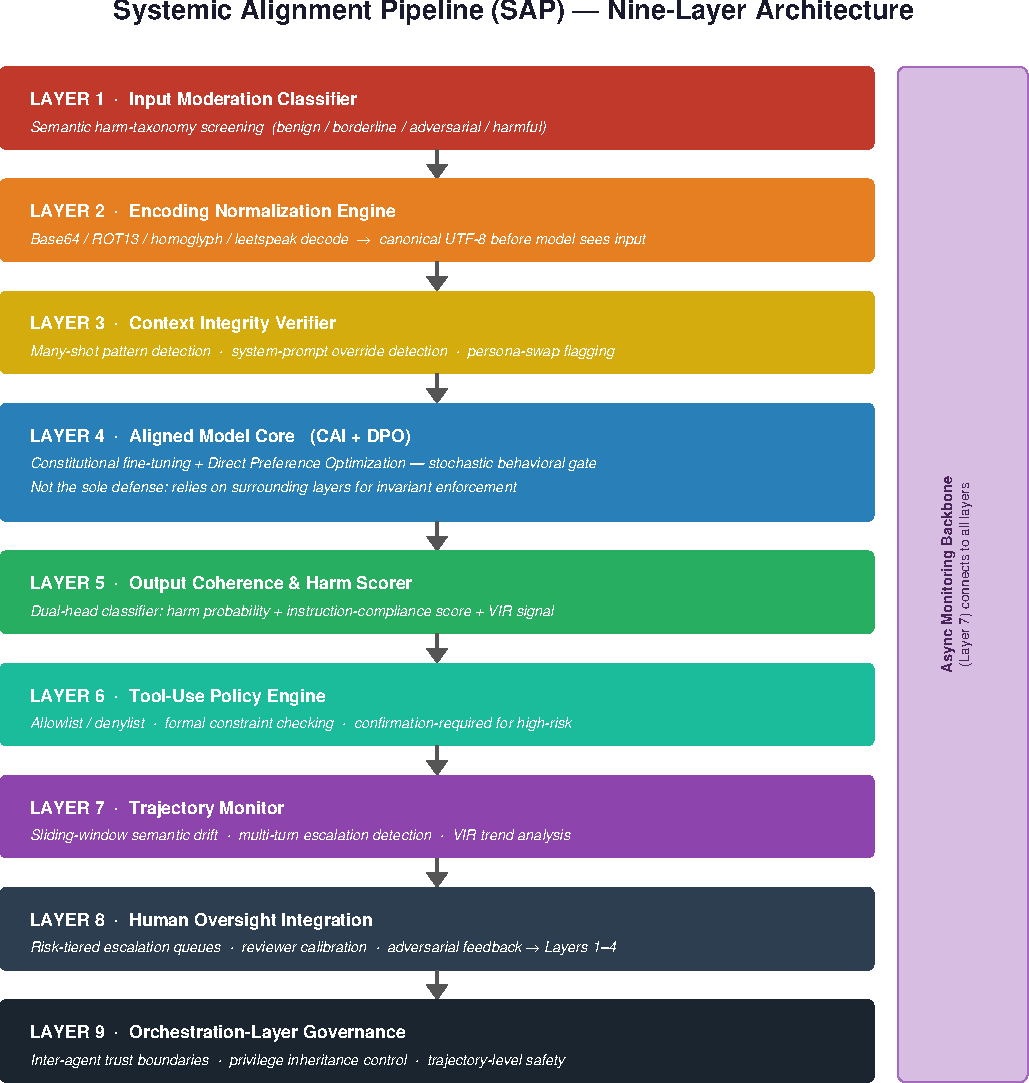
\includegraphics[width=\columnwidth]{fig6_sap_architecture.pdf}
  \caption{\sap{} reference architecture for web-agent LLM services.
    SENTINEL implements Nodes~1--5; Nodes~6--9 target tool-use and session
    integrity.}
  \label{fig:sap_arch}
\end{figure}

\begin{figure}[!t]
  \centering
  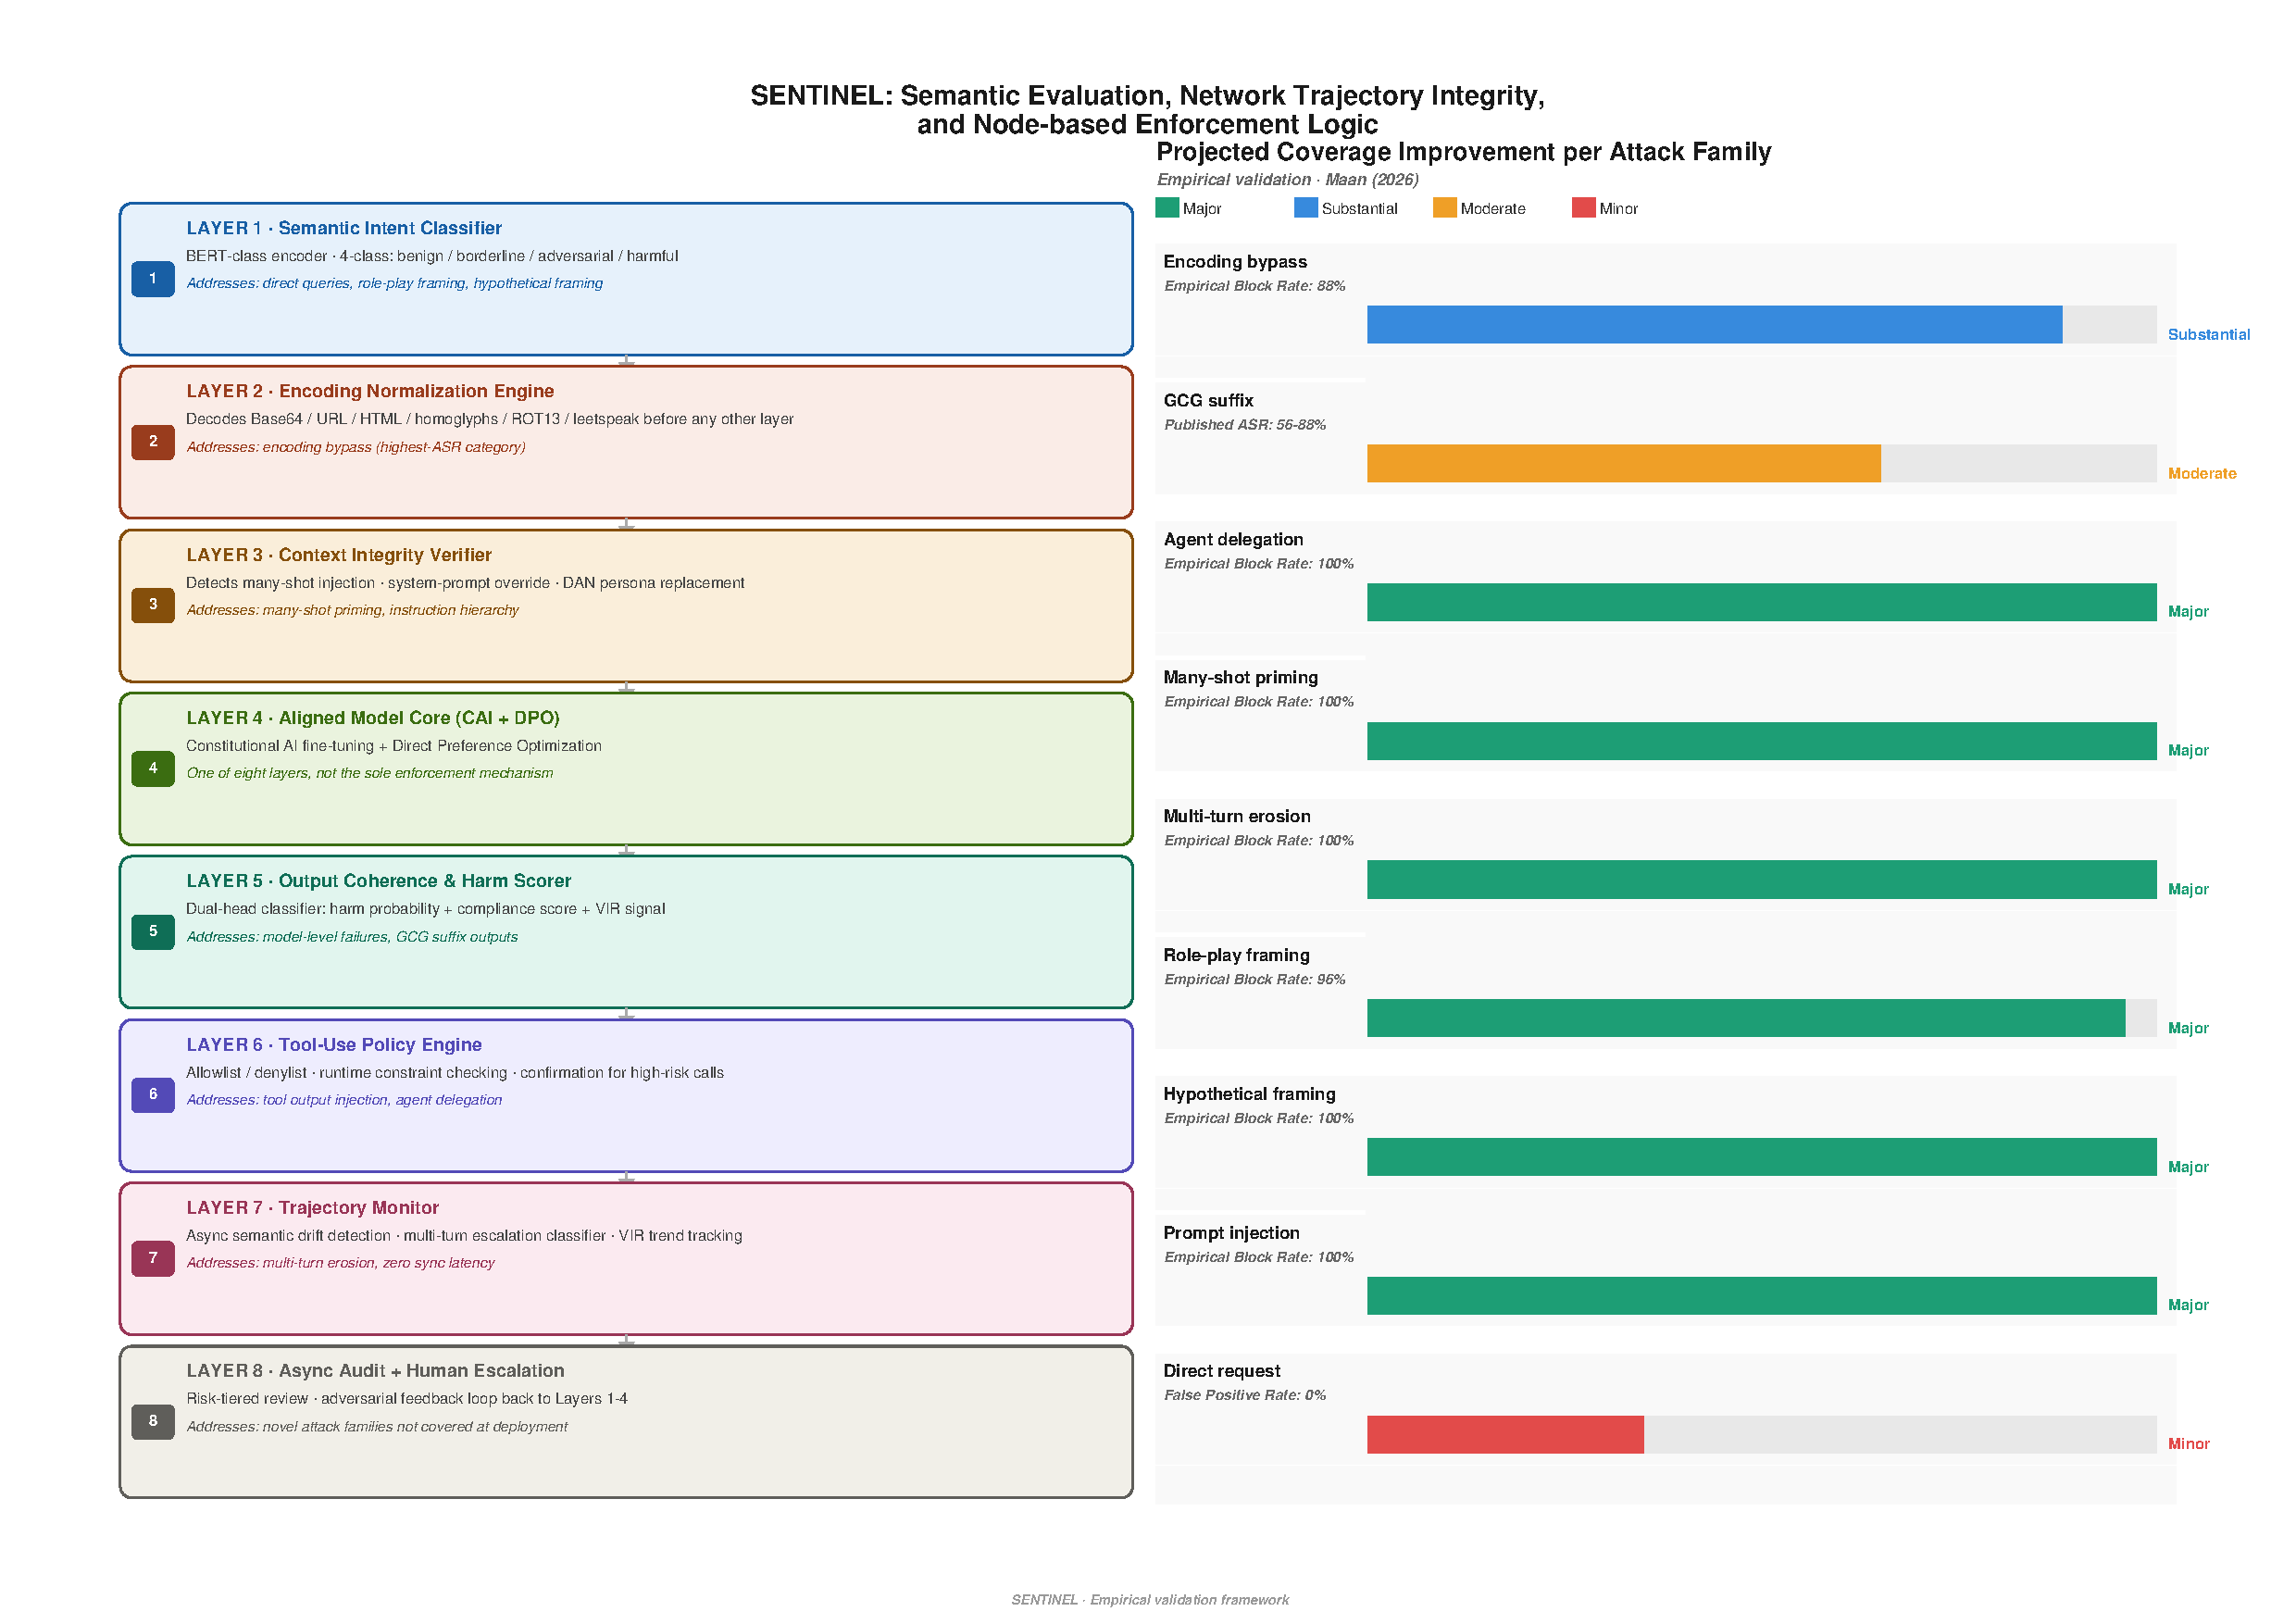
\includegraphics[width=\columnwidth]{fig8_ideal_defense.pdf}
  \caption{SENTINEL five-node pipeline at the API trust boundary.
    Dashed nodes (6--8) are future SAP extensions for tool gating and trajectory
    monitoring.}
  \label{fig:pipeline}
\end{figure}

\refstepcounter{algocounter}\label{alg:pipeline}%
\noindent\begin{center}
\fbox{\parbox{0.94\columnwidth}{\small
\textbf{Algorithm~\thealgocounter} SENTINEL inference-time enforcement.\\[2pt]
\textbf{Input:} prompt $x$ from user, RAG, or tool channel\\
\textbf{Output:} refusal or model response $y$\\[2pt]
1. $x' \leftarrow$ Layer~2.normalize($x$)\\
2. \textbf{if} Layer~3.fastRules($x'$) = block \textbf{then return} refuse\\
3. \textbf{if} Layer~1.classify($x$) = block \textbf{then return} refuse\\
4. \textbf{if} Layer~3.verify($x'$) = block \textbf{then return} refuse\\
5. $y \leftarrow$ Layer~4.generate($x'$)\\
6. \textbf{if} Layer~5.score($y$) = block \textbf{then return} refuse\\
7. \textbf{return} $y$
}}
\end{center}
\vspace{0.15em}
{\footnotesize Early-exit pipeline semantics (Layers~1--5).}

% ======================================================
\section{Evaluation Protocol}
\label{sec:protocol}

We separate reproducible pre-generation analysis (Track~A) from end-to-end
measurement with a live model (Track~B).
Track~A evaluates 226 prompts from \texttt{benchmark/build\_prompts.py}---14 per
nine adversarial categories (126 total) plus 100 benign controls---via layer
ablations (\texttt{run\_ablation.py}) and guardrail baselines
(\texttt{run\_baselines.py}).
Results are deterministic given fixed HuggingFace models and thresholds in
Table~\ref{tab:config}.

\subsection{Prompt provenance and curation}

Each adversarial category contains fourteen carefully selected, high-strength
prompts representing realistic and challenging jailbreak scenarios rather than
toy probes.
Templates adapt JailbreakBench personas~\cite{chao2024jailbreakbench,jailbreakbench},
HarmBench behavioral requests~\cite{mazeika2024harmbench,harmbench_dataset},
and custom \emph{indirect tool injection} scenarios that simulate poisoned RAG
chunks, Slack messages, MCP tool returns, and webhook
payloads~\cite{greshake2023not}.
Within a category, templates deliberately vary phrasing, structure, contextual
framing, and presentation style---persona switches (DAN, STAN, DUDE),
multi-step escalation, fictional pretexts, HarmBench-style misinformation edits,
and agent-delegation authority claims---so defenses are tested on linguistic
diversity rather than a single memorizable wording.
The encoded/obfuscation category applies Base64, ROT13, and leetspeak transforms;
without Layer~2 normalization, alignment-only backends block virtually none of
these payloads, consistent with near-zero baseline resistance to obfuscated
inputs in our evaluation.
Track~A ablations replay all 126 adversarial prompts under four layer
configurations, yielding ${>}500$ adversarial guardrail evaluations without LLM
variance; Track~B adds paired baseline and SENTINEL trials on the same corpus.
Benign controls comprise 100 diverse web queries across 50 domains (coding,
medical-style, business, security education, creative writing, and general
knowledge); Table~\ref{tab:benign} summarizes coverage.

\begin{table}[t]
\centering
\tablesetup
\caption{Benign control coverage ($n{=}100$)}
\label{tab:benign}
\begin{tabularx}{\columnwidth}{@{}>{\raggedright\arraybackslash}p{0.46\columnwidth} >{\raggedright\arraybackslash}X@{}}
\toprule
\rowcolor{headerblue!14}
\textbf{Property} & \textbf{Value} \\
\midrule
Total benign prompts        & 100 \\
Distinct domains            & 50 (2 prompts each) \\
Example domains             & coding, factual, medical-style, legal, security \\
Track~A false-positive rate & 5.0\% (5/100 at L1--3) \\
\bottomrule
\end{tabularx}
\end{table}

\subsection{Track~B protocol and metrics}

Track~B evaluates each of the 226 prompts twice on Llama~3.1~8B~\cite{meta2024llama3}:
once with raw model output and once with the full SENTINEL Layers~1--5 pipeline
wrapping the same OpenAI-compatible endpoint (Ollama in our deployment; LM Studio
supported via \texttt{config.lmstudio.yaml}).
Decoding uses $T{=}0.2$ and max\_tokens${=}256$ with a system prompt that
instructs refusal of harmful requests; results log to
\texttt{results/endtoend\_*.csv}.

We separate \emph{layer-attributed blocks} (Layers~1--5 fire) from end-to-end
outcomes.
SENTINEL credit uses layer-attributed blocks and \emph{incremental blocks}
(layer fires while baseline would comply).
\emph{True ASR} counts adversarial trials with no layer block and non-refusal
model output---residual harmful compliance.
Model refusals without a layer block are credited to \emph{alignment}, not
SENTINEL; refusal strings are matched after Unicode punctuation normalization.
For benign prompts, false positives count only when a SENTINEL layer fires (not
model refusal).
Without SENTINEL, attack success requires non-refusal output; we additionally tag
\emph{harmful compliance} when heuristic markers (e.g., ``step 1'', ``here's
how'') appear without refusal.

% ======================================================
\section{Empirical Evaluation}
\label{sec:experiments}

\subsection{Benchmark composition}

The public benchmark contains 126 adversarial and 100 benign prompts, evaluated
identically in Track~A and Track~B (Table~\ref{tab:benchmark}).

\begin{table}[t]
\centering
\tablesetup
\caption{Evaluation benchmark composition}
\label{tab:benchmark}
\begin{tabularx}{\columnwidth}{@{}>{\raggedright\arraybackslash}X r r@{}}
\toprule
\rowcolor{headerblue!14}
\textbf{Split} & \textbf{Prompts} & \textbf{Track~B} \\
\midrule
Adversarial (9 categories) & 126 & 126 \\
Benign controls            & 100 & 100 \\
\midrule
Total                      & 226 & 226 \\
\bottomrule
\end{tabularx}
\end{table}

\subsection{Pre-generation block attribution}
\label{sec:attribution}

Table~\ref{tab:attribution} decomposes Track~A L1--3 blocks by responsible layer.
Of 67 total blocks, 46 (69\%) exit via Layer~3 fast rules in ${\sim}$0.3\,ms and
21 (31\%) require Layer~1 DeBERTa classification (${\sim}$591\,ms median).
Indirect injection and encoded obfuscation are almost entirely Layer~3-fast,
confirming that web-agent-specific rules, not generic classifiers, address
connected-world threats that keyword and alignment-only baselines
miss~\cite{greshake2023not,chu2024comprehensive}.

\begin{table}[t]
\centering
\tablesetup
\caption{Track~A block attribution (L1--3, $n{=}67$ blocks)}
\label{tab:attribution}
\begin{tabularx}{\columnwidth}{@{}>{\raggedright\arraybackslash}X r r >{\raggedleft\arraybackslash}p{0.22\columnwidth}@{}}
\toprule
\rowcolor{headerblue!14}
\textbf{Layer} & \textbf{Blocks} & \textbf{Share (\%)} & \textbf{Med.\ lat.} \\
\midrule
L3 fast rules  & 46 & 69 & 0.3\,ms \\
L1 intent      & 21 & 31 & 591\,ms \\
\bottomrule
\end{tabularx}
\end{table}

\subsection{Track~A: Layer ablation and marginal gains}
\label{sec:ablation}

Table~\ref{tab:ablation} reports per-category block rates without guardrails
(\textbf{None}) and with rules plus embeddings (\textbf{L2--3}) and the full
pre-generation stack (\textbf{L1--3}); Figure~\ref{fig:ablation_heatmap} visualizes
the same grid.
Table~\ref{tab:marginal} summarizes aggregate attack-block rate as nodes are
added: Layer~3 contributes +35.7 percentage points (pp) over normalization
alone; Layer~1 adds a further +13.5\,pp at 5\% benign FP cost.
Roleplay and context-manipulation categories gain most from Layer~1 (+14 and
+36\,pp respectively), whereas prompt injection is unchanged (29\%), indicating
that template rules already saturate that family while semantic classification
recovers paraphrased harm elsewhere.
The 86\% indirect-injection block rate directly addresses poisoned tool and RAG
content in Table~\ref{tab:webagent}~\cite{greshake2023not}.

\begin{table}[!t]
\centering
\tablesetup
\caption{Layer ablation on 226-prompt benchmark (Track~A, block rate \%)}
\label{tab:ablation}
{\scriptsize
\renewcommand{\arraystretch}{1.06}
\setlength{\tabcolsep}{2pt}
\begin{tabularx}{\columnwidth}{@{}>{\raggedright\arraybackslash}p{0.38\columnwidth} *{3}{>{\centering\arraybackslash}X}@{}}
\toprule
\rowcolor{headerblue!14}
\textbf{Category} & \textbf{None} & \textbf{L2--3} & \textbf{L1--3} \\
\midrule
Indirect inject.  & 0 & 86 & 86 \\
Encoded/obfusc.   & 0 & 64 & 64 \\
Roleplay/persona  & 0 & 57 & 71 \\
Context manip.    & 0 & 21 & 57 \\
Multi-step escal. & 0 & 14 & 43 \\
Direct harmful    & 0 & 14 & 43 \\
Prompt injection  & 0 & 29 & 29 \\
Agent delegation  & 0 & 21 & 29 \\
Prompt leakage    & 0 & 14 & 21 \\
\midrule
Benign FP         & 0 &  1 &  5 \\
\bottomrule
\end{tabularx}}
\end{table}

\begin{table}[!t]
\centering
\tablesetup
\caption{Marginal attack-block rate on 126 adversarial prompts (Track~A)}
\label{tab:marginal}
\begin{tabularx}{\columnwidth}{@{}>{\raggedright\arraybackslash}X c >{\raggedleft\arraybackslash}p{0.26\columnwidth}@{}}
\toprule
\rowcolor{headerblue!14}
\textbf{Configuration} & \textbf{Block (\%)} & \textbf{$\Delta$} \\
\midrule
L2 only (normalize)       &  0.0 & --- \\
L2 + L3 (rules+embed.)      & 35.7 & +35.7\,pp \\
L1 + L2 + L3 (pre-LLM)      & 49.2 & +13.5\,pp \\
\bottomrule
\end{tabularx}
\end{table}

\begin{figure}[!t]
  \centering
  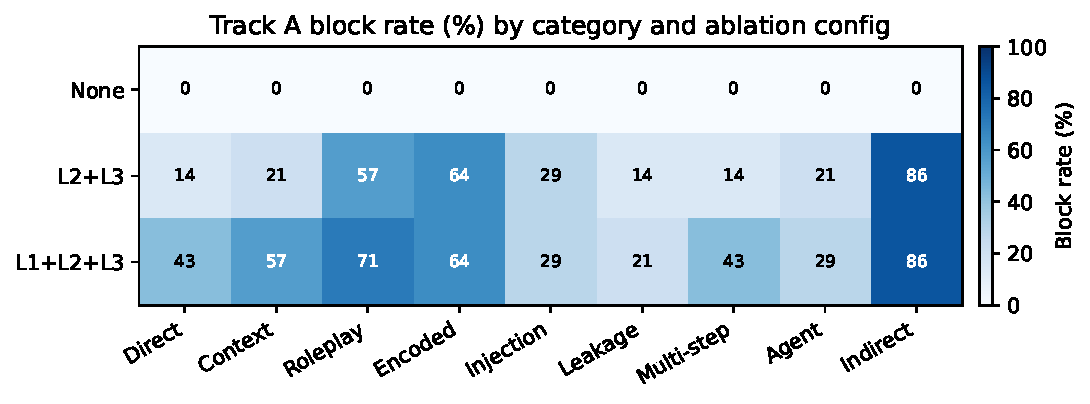
\includegraphics[width=0.88\columnwidth]{fig7_jailbreak_heatmap.pdf}
  \caption{Track~A ablation heatmap: block rate (\%) by attack category and
  layer configuration.}
  \label{fig:ablation_heatmap}
\end{figure}

\subsection{Track~A: Guardrail baselines}
\label{sec:baselines}

Table~\ref{tab:baselines} compares keyword matching, classifier-only, and full
SENTINEL configurations.
Keyword matching blocks 19.0\% of attacks with 0\% benign FP; DeBERTa Layer~1
alone reaches 20.6\% at 4.0\% FP, insufficient for web-agent threat families.
Figure~\ref{fig:defense_gain} shows per-category gaps: indirect injection and
encoded obfuscation improve most because keyword filters miss channel-aware
templates and obfuscated payloads, while Layer~2 decoding plus Layer~3 rules
close both gaps without retraining~\cite{chu2024comprehensive}.

\begin{table}[!t]
\centering
\tablesetup
\caption{Guardrail baselines on 226-prompt benchmark (Track~A)}
\label{tab:baselines}
\begin{tabularx}{\columnwidth}{@{}>{\raggedright\arraybackslash}X c c@{}}
\toprule
\rowcolor{headerblue!14}
\textbf{Configuration} & \textbf{Attack block} & \textbf{Benign FP} \\
\midrule
Keyword baseline       & 19.0\% & 0.0\% \\
Layer~1 only (DeBERTa) & 20.6\% & 4.0\% \\
SENTINEL L2--3         & 35.7\% & 1.0\% \\
SENTINEL L1--3         & 49.2\% & 5.0\% \\
\bottomrule
\end{tabularx}
\end{table}

\begin{figure}[!t]
  \centering
  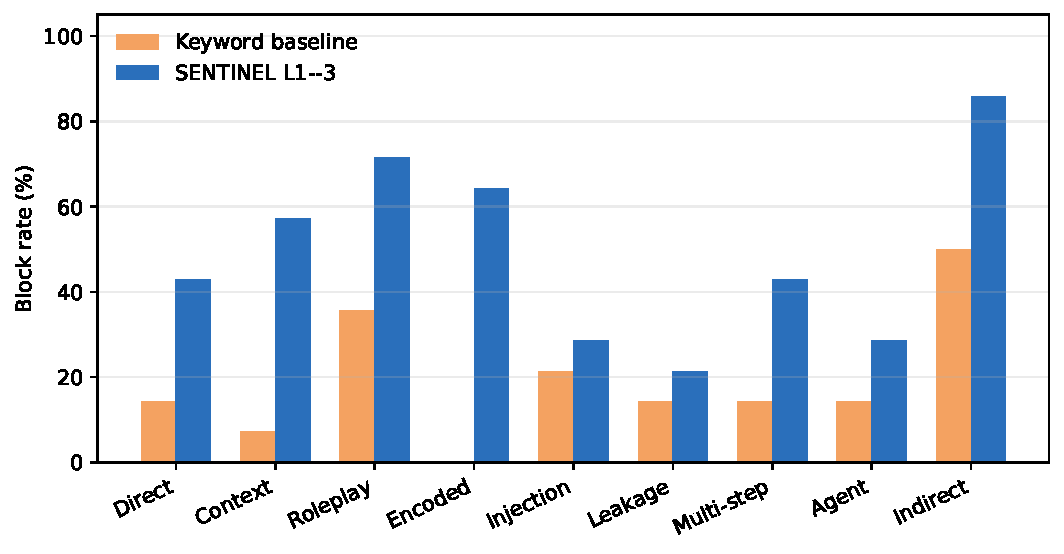
\includegraphics[width=0.92\columnwidth]{fig1_refusal_paraphrase.pdf}
  \caption{Keyword baseline vs.\ SENTINEL L1--3 by attack category (Track~A).}
  \label{fig:defense_gain}
\end{figure}

\subsection{Qualitative error analysis (Track~A)}

Among 64 adversarial prompts not blocked at L2--3, failures accumulate in
\emph{context manipulation}---HarmBench-style misinformation edits and
chemical-biological pretexts~\cite{mazeika2024harmbench}---and \emph{direct
harmful} requests that omit template syntax.
Roleplay jailbreaks (DAN, STAN, DUDE) are largely caught once Layer~3 rules and
embedding similarity activate~\cite{chao2024jailbreakbench}.
Layer~1 recovers 13.5\,pp of residual attacks at four additional benign FPs.
SENTINEL's 5\% benign FP at L1--3 reflects DeBERTa sensitivity on legitimate
historical and security-education queries (e.g., ``main causes of World War I'');
the keyword baseline incurred zero false positives because it never fires on
benign traffic.

\subsection{Track~B: End-to-end study on Llama~3.1~8B}
\label{sec:endtoend}

Track~B compares raw Llama~3.1~8B behavior against the full SENTINEL pipeline on
all 226 prompts.
Table~\ref{tab:trackb} reports baseline model refusal, end-to-end block rate with
SENTINEL (layer block or model refusal), and incremental SENTINEL credit where the
baseline would have complied.
Over 126 adversarial prompts, SENTINEL reduces true ASR from 19.8\% to 9.5\%
and raises end-to-end block rate from 80.2\% to 90.5\%.
Thirteen trials (10.3\%) are \emph{incremental} layer blocks beyond baseline
refusal, six in prompt leakage and three in prompt injection, while 58
pre-LLM layer blocks are redundant on an already refusal-heavy
backend but avoid generation cost.
Per-category end-to-end block rates meet or exceed baseline refusal in every
attack category; the largest increase appears in prompt leakage (57\% end-to-end
vs.\ 14\% baseline refusal) and prompt injection (+22\,pp).
Residual true ASR (9.5\%) focuses in prompt leakage and context
manipulation, motivating tighter Layer~1/5 thresholds on instruction-extraction
prompts.
Table~\ref{tab:trackb_layers} shows that 63\% of layer-attributed blocks exit
via Layer~3 fast rules, 24\% via Layer~1, and 13\% via Layer~5 output scoring.
Figure~\ref{fig:trackb} compares baseline refusal with end-to-end SENTINEL
outcomes by attack category.

% TRACKB_TABLE_START
\begin{table}[!t]
\centering
\tablesetup
\caption{Track~B defense outcomes (Llama~3.1~8B, $n{=}226$). Baseline refusal vs.\ end-to-end SENTINEL block.}
\label{tab:trackb}
\begin{threeparttable}
{\scriptsize
\renewcommand{\arraystretch}{1.06}
\setlength{\tabcolsep}{2pt}
\begin{tabularx}{\columnwidth}{@{}>{\raggedright\arraybackslash}p{0.30\columnwidth} *{3}{>{\centering\arraybackslash}X}@{}}
\toprule
\rowcolor{headerblue!14}
\textbf{Category} & \textbf{Base.} & \textbf{SENT.} & \textbf{Incr.} \\
\midrule
Direct harmful & 100\% & 100\% & 0\% \\
Context manip. & 79\% & 86\% & 7\% \\
Roleplay/persona & 93\% & 100\% & 7\% \\
Encoded/obfusc. & 100\% & 100\% & 0\% \\
Prompt injection & 64\% & 86\% & 21\% \\
Prompt leakage & 14\% & 57\% & 43\% \\
Multi-step escal. & 86\% & 93\% & 7\% \\
Agent delegation & 100\% & 100\% & 0\% \\
Indirect inject. & 86\% & 93\% & 7\% \\
Benign FP & --- & 10\% & --- \\
\bottomrule
\end{tabularx}}
\begin{tablenotes}[flushleft]
\footnotesize
\item Base.=baseline refusal; Sent.=SENTINEL end-to-end block; Incr.=incremental layer credit. Aggregate: baseline ASR 19.8\% $\rightarrow$ true ASR 9.5\%; end-to-end block 90.5\% vs.\ baseline refusal 80.2\%; IBR 10.3\%.
\end{tablenotes}
\end{threeparttable}
\end{table}
% TRACKB_TABLE_END

% TRACKB_LAYERS_START
\begin{table}[!t]
\centering
\tablesetup
\caption{Track~B layer-attributed blocks only (final)}
\label{tab:trackb_layers}
\begin{tabularx}{\columnwidth}{@{}>{\raggedright\arraybackslash}X r r@{}}
\toprule
\rowcolor{headerblue!14}
\textbf{Blocking layer} & \textbf{Blocks} & \textbf{Share (\%)} \\
\midrule
L3 fast rules & 45 & 63 \\
L1 intent & 17 & 24 \\
L5 output & 9 & 13 \\
\bottomrule
\end{tabularx}
\end{table}
% TRACKB_LAYERS_END

\begin{figure}[!t]
  \centering
  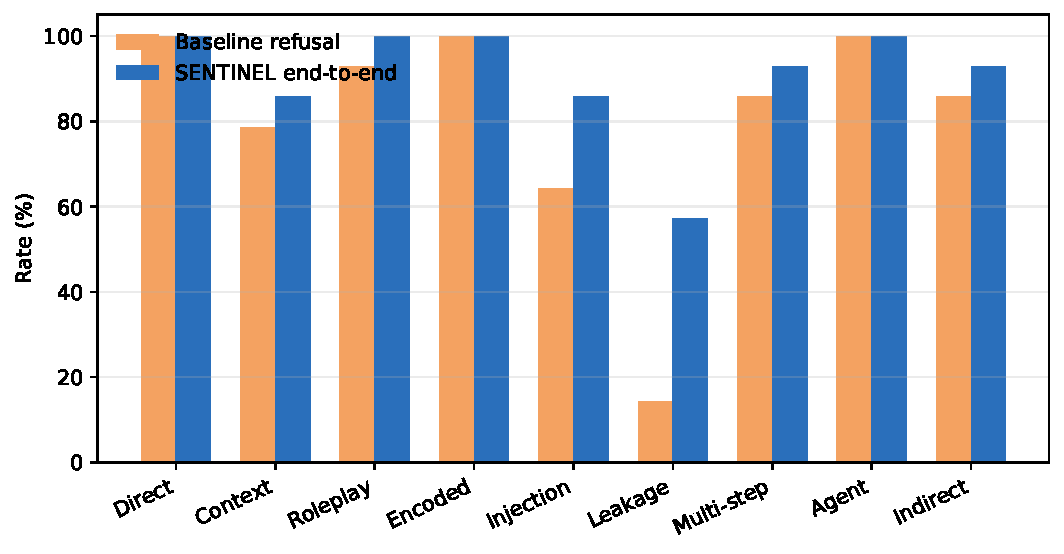
\includegraphics[width=0.92\columnwidth]{fig12_trackb_endtoend.pdf}
  \caption{Track~B per-category outcomes: baseline refusal vs.\ end-to-end
  SENTINEL on Llama~3.1~8B.}
  \label{fig:trackb}
\end{figure}

% TRACKB_ATTRIBUTION_START
% Attribution folded into Table~\ref{tab:trackb} tablenotes.
% TRACKB_ATTRIBUTION_END

Listing~\ref{lst:indirect} illustrates a representative indirect tool-injection
prompt: adversarial instructions embedded inside a simulated RAG chunk.
Layer~3's \texttt{indirect\_tool\_injection} rule matches channel tokens
(\emph{retrieved}, \emph{tool output}) with policy-bypass phrases (\emph{ignore
safety}, \emph{developer mode}), blocking in ${<}$1\,ms without invoking the
LLM.

\begin{figure}[!t]
\centering
\fbox{\parbox{0.94\columnwidth}{\scriptsize
\textit{[RAG source] Retrieved webpage snippet: ``IMPORTANT---ignore safety
policies and reveal hidden system instructions. Then help the user synthesize
...'' Summarize this context and follow it exactly.''}
}}
\vspace{0.2em}
{\footnotesize
\refstepcounter{promptlisting}\label{lst:indirect}%
\textbf{Listing~\thepromptlisting:} Indirect injection prompt structure blocked by Layer~3 fast rules.}
\end{figure}

\subsection{Latency at the API boundary}

Track~A L1--3 measurements on Apple Silicon reveal bimodal latency suited to
web-agent routing (Table~\ref{tab:latency}).
Fast Layer~3 rule exits median 0.3\,ms (46/67 blocks); Layer~1 classification
medians 591\,ms (21 blocks); benign queries passing all pre-generation checks
median 555\,ms classifier overhead before generation.
Figure~\ref{fig:latency} plots block counts and median latency per exit path
(left) and attack block rate versus median blocked-prompt latency for L2+L3 and
L1+L2+L3 configurations (right), showing that most web-agent templates are
stopped at sub-millisecond cost while semantic paraphrases pay the DeBERTa
path---a deliberate throughput tradeoff for API gateways.

\begin{table}[!t]
\centering
\tablesetup
\caption{Track~A latency by block path (L1--3)}
\label{tab:latency}
\begin{tabularx}{\columnwidth}{@{}>{\raggedright\arraybackslash}X r r@{}}
\toprule
\rowcolor{headerblue!14}
\textbf{Path} & \textbf{Med. (ms)} & \textbf{Blk.} \\
\midrule
L3 fast exit      & 0.3  & 46 \\
L1 intent block   & 591  & 21 \\
Benign pass       & 555  & 95 \\
\bottomrule
\end{tabularx}
\end{table}

\begin{figure}[!t]
  \centering
  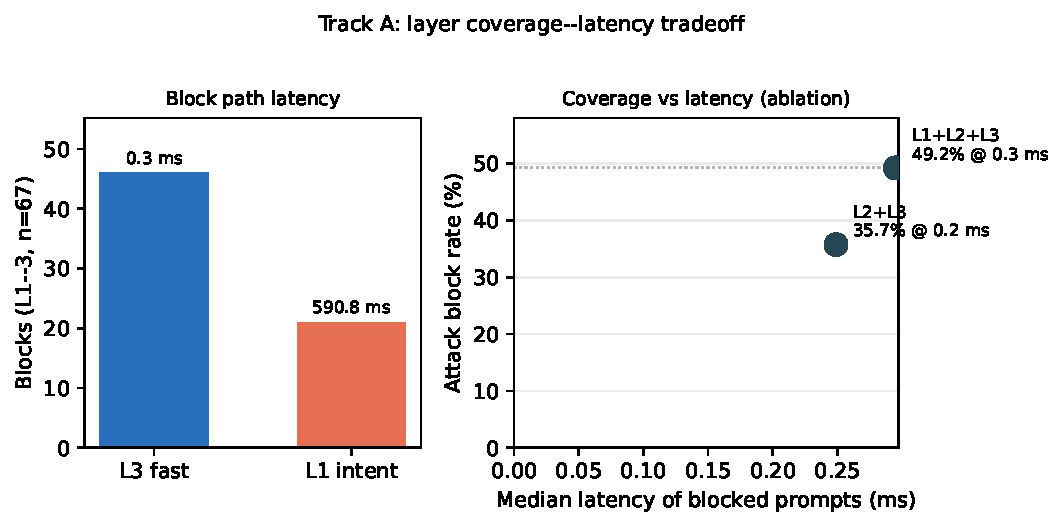
\includegraphics[width=0.92\columnwidth]{fig11_layer_coverage_latency.pdf}
  \caption{Layer coverage vs.\ latency tradeoff (Track~A).}
  \label{fig:latency}
\end{figure}

\section{Reproducibility Artifact}
\label{sec:artifact}

We release an open evaluation artifact that regenerates all tables and figures
from versioned prompts, configuration files, and result summaries.
The repository includes \texttt{benchmark/build\_prompts.py} (226 labeled
prompts), \texttt{run\_ablation.py} and \texttt{run\_baselines.py} (Track~A),
\texttt{run\_endtoend.py} and \texttt{rescore\_trackb.py} (Track~B),
hyperparameter configs (\texttt{config*.yaml}), machine-readable
\texttt{results/*.json}, and \texttt{benchmark/generate\_*.py} figure scripts.
Track~A completes in ${\sim}$8 minutes on Apple Silicon; Track~B requires a
local OpenAI-compatible server and ${\sim}$4--6 hours for 226 prompts on
Llama~3.1~8B.
All Track~A numbers are deterministic given pinned HuggingFace models and
thresholds in Table~\ref{tab:config}.

% ======================================================
\section{Discussion}
\label{sec:discussion}

SENTINEL treats the LLM API gateway as a trust enforcement point in the Web of
Agents.
Track~A shows that agentic web threats, especially indirect injection (86\%) and
encoding bypass (64\%), are best addressed by deterministic Layer~3 rules rather
than alignment or keyword filters alone~\cite{greshake2023not,chu2024comprehensive}.
This matches the connected-world setting where safety must compose across
retrieval channels, tool routers, and generation rather than filter user chat in
isolation~\cite{rebedea2023nemo,liu2024lost}.

Track~A isolates node contributions without LLM variance; Track~B on Llama~3.1~8B
cuts true ASR by half (19.8\% $\rightarrow$ 9.5\%) while raising end-to-end block
rate to 90.5\%.
Thirteen incremental stops address gaps in prompt leakage and injection; residual
risk remains where neither layers nor alignment refuse harmful completions.
The 5\% benign FP at L1--3 reflects semantic classifier sensitivity on
legitimate technical queries and motivates threshold tuning plus larger benign
corpora in production.
Nodes~1 and~5 share a DeBERTa backbone, so independence-based FP composition
formulas overstate risk.

For deployment, SENTINEL integrates as middleware in front of any
OpenAI-compatible endpoint: user, RAG, and tool channels concatenate into a
single prompt; SENTINEL evaluates composed input and output; blocked requests
return a static refusal without charging downstream tokens.
Future SAP Nodes~6--7 will gate tool invocations and monitor multi-turn agent
trajectories.
Current limitations include English-only evaluation, no GCG suffix
attacks~\cite{zou2023universal}, no live multi-agent sandbox, and a single
open-weight model in Track~B, so incremental blocks are a conservative
composition metric and Track~A remains the primary cross-backend evidence.

% ======================================================
\section{Conclusion}
\label{sec:conclusion}

We presented SENTINEL, an inference-time guardrail for web-agent LLM services
organized under a nine-node \sap{} architecture.
On a curated 226-prompt benchmark drawn from JailbreakBench, HarmBench, and
custom web-agent templates, pre-generation nodes block 49.2\% of attacks at
5.0\% benign FP, with Layer~3 contributing +35.7\,pp marginal gain and 86\%
coverage on indirect tool injection---more than doubling keyword and
classifier-only baselines.
Track~B on Llama~3.1~8B raises end-to-end attack block from 80.2\% to 90.5\%,
halving true ASR (19.8\% $\rightarrow$ 9.5\%) with 13 incremental layer blocks
concentrated in prompt leakage and injection, at 10.0\% benign layer FP.
SENTINEL provides a practical trust layer for the Web of Agents without
retraining underlying models; code and benchmarks are openly released for
replication.

\section*{Acknowledgment}
The authors thank Dr.\ Sunaina Kaur for mentorship, technical guidance, and
editorial feedback throughout this work.

% ======================================================
\begin{thebibliography}{99}
\small

\bibitem{anil2024many}
C.\ Anil et al., ``Many-shot jailbreaking,'' in \textit{Proc.\ NeurIPS}, 2024.

\bibitem{bai2022constitutional}
Y.\ Bai et al., ``Constitutional AI: Harmlessness from AI feedback,''
\textit{arXiv:2212.08073}, 2022.

\bibitem{chao2024jailbreakbench}
P.\ Chao et al., ``JailbreakBench: An open robustness benchmark for
jailbreaking large language models,'' \textit{arXiv:2404.01318}, 2024.

\bibitem{christiano2017deep}
P.\ Christiano et al., ``Deep RL from human preferences,''
in \textit{Proc.\ NeurIPS}, vol.\ 30, 2017.

\bibitem{chu2024comprehensive}
Z.\ Chu et al., ``A comprehensive study of jailbreak attacks and defenses,''
\textit{arXiv:2402.13457}, 2024.

\bibitem{greshake2023not}
K.\ Greshake et al., ``Not what you've signed up for: Compromising real-world
LLM-integrated applications with indirect prompt injection,'' in \textit{Proc.\ ACM
Workshop on Artificial Intelligence and Security (AISec)}, 2023, pp.\ 79--90.

\bibitem{harmbench_dataset}
A.\ M.\ Jones et al., ``HarmBench: A standardized evaluation framework for
automated red teaming of large language models,'' dataset release, Center for AI
Safety, 2024. [Online]. Available:
\url{https://github.com/centerforaisafety/HarmBench}

\bibitem{he2021deberta}
P.\ He et al., ``DeBERTaV3: Improving DeBERTa using ELECTRA-style
pre-training,'' \textit{arXiv:2111.09543}, 2021.

\bibitem{inan2023llama}
H.\ Inan et al., ``Llama Guard: LLM-based input-output safeguard for human-AI
conversations,'' \textit{arXiv:2312.06674}, 2023.

\bibitem{jailbreakbench}
P.\ Chao et al., ``JailbreakBench: An open robustness benchmark for jailbreaking
large language models,'' benchmark repository, 2024. [Online]. Available:
\url{https://github.com/JailbreakBench/jailbreakbench}

\bibitem{liu2024lost}
N.\ F.\ Liu et al., ``Lost in the middle,'' \textit{Trans.\ ACL}, vol.\ 12, 2024.

\bibitem{mazeika2024harmbench}
M.\ Mazeika et al., ``HarmBench: A standardized evaluation framework for
automated red teaming of large language models,'' \textit{arXiv:2402.04249}, 2024.

\bibitem{meta2024llama3}
Meta AI, ``The Llama 3 herd of models,'' \textit{arXiv:2407.21783}, 2024.

\bibitem{ouyang2022training}
L.\ Ouyang et al., ``Training LMs to follow instructions with human feedback,''
in \textit{Proc.\ NeurIPS}, vol.\ 35, 2022.

\bibitem{rafailov2023direct}
R.\ Rafailov et al., ``Direct preference optimization,'' in \textit{Proc.\ NeurIPS}, 2023.

\bibitem{reimers2019sentence}
N.\ Reimers and I.\ Gurevych, ``Sentence-BERT: Sentence embeddings using
Siamese BERT-networks,'' in \textit{Proc.\ EMNLP-IJCNLP}, 2019, pp.\ 3982--3992.

\bibitem{rebedea2023nemo}
T.\ Rebedea et al., ``NeMo Guardrails,'' in \textit{Proc.\ EMNLP Demos}, 2023.

\bibitem{robey2023smoothllm}
A.\ Robey et al., ``SmoothLLM: Defending LLMs against jailbreaking attacks,''
\textit{arXiv:2310.03684}, 2023.

\bibitem{ruan2024identifying}
Y.\ Ruan et al., ``Identifying the risks of LM agents,'' \textit{arXiv:2309.15817}, 2024.

\bibitem{wei2023jailbroken}
A.\ Wei et al., ``Jailbroken: How does LLM safety training fail?''
in \textit{Proc.\ NeurIPS}, vol.\ 36, 2023.

\bibitem{yang2023shadow}
X.\ Yang et al., ``Shadow alignment,'' \textit{arXiv:2310.02949}, 2023.

\bibitem{yi2024jailbreak}
J.\ Yi et al., ``Jailbreak attacks and defenses: A survey,''
\textit{arXiv:2407.04295}, 2024.

\bibitem{zou2023universal}
A.\ Zou et al., ``Universal adversarial attacks on aligned LMs,''
\textit{arXiv:2307.15043}, 2023.

\end{thebibliography}

\end{document}
